 \documentclass[12pt]{spieman}  % 12pt font required by SPIE;
%\documentclass[a4paper,12pt]{spieman}  % use this instead for A4 paper
\include{moritz}
\usepackage{amsmath,amsfonts,amssymb}
\usepackage{graphicx}
\usepackage{setspace}
\usepackage{tocloft}
\usepackage{gensymb}
\usepackage{lineno}
\linenumbers

\title{A concept for a critical-angle transmission grating spectrometer for the AXIS probe}
\author[a]{Hans M. G\"unther}
\author[a]{David A. Principe}
\author[a,b]{Ralf K. Heilmann}
\author[c]{Peter Cheimets}
\author[c]{Edward Hertz}
\author[c]{Randall Smith}
\affil[a]{MIT Kavli Institute for Astrophysics and Space Research, Massachusetts Institute of Technology, Cambridge, MA 02139, USA}
\affil[b]{Space Nanotechnology Laboratory, Massachusetts Institute of Technology, Cambridge, MA 02139, USA}
\affil[c]{Center for Astrophysics $|$ Harvard \& Smithsonian, 60 Garden Street, Cambridge, MA 02138, USA}

\renewcommand{\cftdotsep}{\cftnodots}
\cftpagenumbersoff{figure}
\cftpagenumbersoff{table}
\begin{document}
\maketitle

\begin{abstract}
The Advanced X-ray Imaging Satellite (AXIS) is a probe-class mission study in response to the 2020 Astrophysics Decadal Survey, which recommended two competed probe-class missions, one of which shall be an X-ray probe with high spatial and spectral resolution. AXIS will feature large collecting area with a point-spread-function (PSF) of order 1-2 arcsec. We describe a possible X-ray grating spectrometer (XGS) that could be added to AXIS with minimal design changes to the telescope itself at a cost of just a few percent of the total mission budget. The XGS would be based on critical-angle transmission (CAT) gratings, a technology already matured for Arcus and Lynx. Using detailed ray-tracing, we investigate several options for sub-aperturing which provide a trade-off between effective area and spectral resolving power.
Depending on how much of the full aperture is covered with gratings (e.g., 17-100\%), we find a high spectral resolving power up to $\lambda/\Delta\lambda 5000-7000$ can be achieved with effective area up to 2000~cm$^2$ in the soft X-ray band (1.5-3.5 nm).
An important benefit of CAT gratings is that they are mostly transparent at high energies, and thus hard X-rays can still be used for simultaneous imaging spectroscopy. We study different grating sizes and other enhancements, but even in the basic configuration an XGS can be added to AXIS to provide the high-resolution spectral capabilities that the  Astrophysics Decadal Survey calls for. Our ray-tracing shows that this concept is mature and can be added to AXIS with minimal impact on other instruments. We discuss one exemplary science case that would be enabled by the XGS.

\end{abstract}

\keywords{ray-tracing, X-ray optics, critical-angle transmission grating, AXIS, Rowland torus, grating spectroscopy}

% Include email contact information for corresponding author
{\noindent \footnotesize\textbf{*}Hans M. G\"unther,  \linkable{hgunther@mit.edu} }

% Activate this before submission
%\begin{spacing}{2}   % use double spacing for rest of manuscript
% But for display on the screen in overleaf it is much easier to look at single spaced
% text because it does not require constant scrolling
\begin{spacing}{1}



\section{Introduction}
\label{sect:introduction}
The NASA 2020 Decadal Survey ``Pathways to Discovery in Astronomy and Astrophysics for the 2020s''\cite{2021pdaa.book.....N} recommends the implementation of a Probe-class line of missions with the first mission to the selected from proposals for Far-Infrared or X-ray missions. Probe-class missions are located between NASA's medium explorer (MIDEX) programs and multi-billion dollar flagship missions. The Advanced X-ray Imaging Satellite (AXIS) was proposed as a white paper \cite{2019BAAS...51g.107M} to the decadal survey and the concept has been continuously developed since. AXIS would use a Si meta-shell approach to nest a large number of precisely formed Si mirrors to achieve a high effective area about two orders of magnitude better than Chandra, while maintaining a Point-Spread-Function (PSF) of order 1-2 arcsec over a much larger field of view. Mirrors and detectors are optimized for similar energies as Chandra and XMM-Newton, from about 0.3 to 10~keV.

With these characteristics, AXIS will deliver much sharper images than the planned Athena mission\cite{doi:10.1117/12.2188988,doi:10.1117/12.2057347}. AXIS mission science would target a few specific science cases, such as galaxy evolution and feedback, the growth of black holes, and active galactic nuclii (AGN) in the high-redshift universe, but importantly function as a proposal-driven observatory that provides unique capabilities to a large range of science questions.

AXIS imaging requires just the mirror and an imaging spectrometer such as a CCD array at the focal plane. The CCD (or similar device) will provide low-resolution spectroscopic capabilities, but particularly in the soft-X-ray band the best CCD energy resolution is only of order 70~eV. In this work, we show that a grating spectrometer can outperform a CCD in soft X-rays by more than two orders of magnitude in terms of resolving power and thus enable fundamentally new science investigations that resolve emission or absorption lines profiles from stars, black holes, and galaxies, or detect weak absorption lines from e.g.\ the warm-hot intergalactic medium super-imposed on background continuum sources. While microcalorimeters achieve an energy resolution of a few eV, in the soft X-ray band that only corresponds to a resolving power of order 100 and microcalorimeters require extensive cooling and engineering at high cost, which puts them out of reach for AXIS\cite{10.1117/1.JATIS.1.1.014006,2022IJMPD..3130001T}.

The initial AXIS design does not include a grating spectrometer, but we show here that one can be added in future design iterations.
We present a design based on critical-angle transmission (CAT) gratings, which can be mounted behind the mirror, either permanently or on a mechanism that folds in and out as with the Chandra High and Low Energy Transmission Gratings (HETG\cite{2005PASP..117.1144C} and LETG\cite{2000APS..APR.J8005B}), which have been operated successfully for over 24 years. CAT gratings are blazed and diffract most light to just one side, where additional CCDs would be located to observe the diffracted photons.

CAT gratings\cite{heilmann:11,doi:10.1117/12.2188525} are one of the enabling technologies for the Arcus X-ray grating spectrometer Explorer mission\cite{doi:10.1117/12.2272818}, which was proposed as a MIDEX mission, but not selected by NASA. The MIDEX version of Arcus was designed for $R > 3500$ with $A_\mathrm{eff}$ up to $350\;\mathrm{cm}^2$ in the band between 1.2 and 5.0 nm wavelength. CAT gratings were also selected for the design reference mission for an XGS on Lynx\cite{10.1117/1.JATIS.5.2.021003}, one of the four mission concepts studied in detail before the 2020 Decadal survey\cite{10.1117/1.JATIS.5.2.021001}.

We have performed extensive ray-trace studies for both Arcus\cite{doi:10.1117/12.2273011,guntherarcus} and Lynx/XGS\cite{10.1117/1.JATIS.5.2.021003}. In particular the Lynx/XGS is quite similar to the proposed XGS for AXIS that we describe here and we refer the reader to Ref~\citenum{10.1117/1.JATIS.5.2.021003} for aspects of the design and alignment tolerances not fully covered in this article.
We first present an example for the type of science investigation that can be addressed with AXIS/XGS and not with any other existing or approved instrument; in the later sections we describe the layout of AXIS/XGS and model its performance through ray-tracing.

\section{A science example}
AXIS/XGS will deliver a resolving power 5-10 times higher than any instrument ever flown and simultaneously provides orders of magnitude improvement in effective area compared to the gratings on Chandra and XMM-Newton. Because of the much improved PSF over XMM-Newton, AXIS/XGS can disentangle spectra from moderately crowded fields and obtain many grating spectra at once, when looking at, e.g.\ a stellar cluster.
With this advancement, we can expect ground-breaking results in different fields of astrophysics. Here, we want to just present one example.

Most stars form from molecular clouds in gravitationally bound clusters.  In the early stages of star formation before about 10~Myrs of age, protostars increase their mass by accumulating (accreting) gas and dust from their surrounding molecular cloud. Over time, gravitational contraction causes a star to spin up resulting in the formation of a circumstellar disk\cite{2000ApJ...531..350M} and a powerful magnetic dynamo\cite{1984ApJ...279..763N}. Stellar magnetic fields generated by these dynamos play an essential role in young stellar evolution as they facilitate the transfer of angular momentum between the star-disk system\cite{2013A&A...556A..36G}. Moreover, X-rays generated by magnetically-heated coronal plasma can affect circumstellar disk chemical evolution \cite{2013ApJ...766....8A} and the photoevaporative dispersal of the disk\cite{2014prpl.conf..475A}, constraining the available time for planet formation. Recent models show the disk-wind mass loss rate is dominated by irradiation from 'soft' X-rays between 0.1 - 1.0 keV\cite{2021MNRAS.508.1675E}.

\begin{figure} [ht]
  \begin{center}
  %\begin{tabular}{c} %% tabular useful for creating an array of images
  \includegraphics[width=0.8\textwidth]{dave_axis_fig2}
  %\end{tabular}
  \end{center}
  \caption {\label{fig:science}
  \emph{Top:} Chandra High Energy Transmission Gratings (HETGS) observation (ObsID 8895)  of the Orion Nebula Cluster star-forming region energy filtered between 0.5 - 8.0 keV. The color in the image is scaled logarithmically and has been smoothed to emphasize the dispersed grating events. In the HETGS layout, each source dispersed the spectrum in an X shape on the detector. Several dispersed spectra can be seen. This 25 ks observation demonstrates the power of an instrument capable of achieving high spatial and spectral resolution for a dense region of point sources. Due to Chandra's poor effective area compared to that proposed for AXIS, only the brightest few sources near the aim-point in the image produce enough counts for detailed high resolution spectral fitting. \emph{Bottom:} Conceptual AXIS imaging and spectral array configuration to be used with CAT gratings. The exact number and dimensions of the detectors on the focal plane depends on the devices chosen, but approximate distances and dimensions are given (not to scale in the sketch). Light from the stars on the imaging array is dispersed and a spectral array is placed where grating efficiencies are highest (solid lines); there is a gap between the direct imaging detector and the spectral array where the signal is weak (dashed lines) and thus no detectors are needed. Dispered spectra from several bright sources can be observed at the same time.
  }
\end{figure}

As a result of their rapid rotation and magnetic dynamos, young pre-main sequence stars are relatively bright X-ray sources with $\sim$100 times the L$_{X}$/L$_{bol}$ of their more-evolved spectral counterparts on the main sequence. While thousands of nearby young stars have been imaged with X-ray observatories such as Chandra, XMM-Newton and ROSAT, much of the physical information provided by these 'soft' (0.3-2 keV) emission-line dominated sources is indistinguishable when observed with the poor spectral resolution of CCD imaging provided by these observatories. Both Chandra and XMM-Newton have grating instruments to disperse photons achieving resolving powers of $\sim$1000.  Stellar spectra at these high resolutions provide important temperature and plasma density diagnostics capable of unambiguously characterizing the complex multi-temperature components that make up stellar coronae\cite{2001ApJ...559.1135H}. In particular, the temperature- and density-sensitive lines of H-like and He-like ions, can be used to distinguish between the hot, low-density dynamo-generated coronal emission components and 'cool' $\sim$ 3MK high density accretion shock plasma from material funneled along magnetic field lines from the disk onto the star\cite{2002ApJ...567..434K}.  While these instruments have provided a tantalizing view of the underlying physics governing about a dozen young star-disk systems, the poor effective area and extended PSF size off-axis of these telescopes limits our ability to observe pre-mains sequence stellar physics at the age of planet formation to only the nearest and brightest young stars\cite{2002ApJ...567..434K,2006A&A...459L..29G,2007ApJ...671..592H,2007A&A...468..443T}.


There are two primary features of AXIS that, if leveraged with the inclusion of CAT gratings, can extend our current set of quality high resolution X-ray spectra of young stars from a few dozen to more than several hundred. This instrument design would be ideal for obtaining dozens of high-resolution X-ray spectra of young pre-MS stars in a single observation of a young stellar cluster (see Figure~\ref{fig:science}). These observations could be performed for all nearby stellar clusters easily providing hundreds of high quality X-ray spectra over a much larger mass and age sample than the current dozen young stars achieve. Building large samples of X-ray spectra for stars within a particular stellar cluster would finally allow us to compare plasma characteristics as a function of stellar age, mass, natal molecular cloud abundance and metallicity.

Moreover, the proposed high effective area of AXIS would unlock a brand new science case for studying planet-formation. Planet-forming circumstellar disks absorb soft X-rays imprinting in the high resolution stellar X-ray spectrum a signature which can be used to unambiguously determine the abundance of line-of-sight circumstellar disk oxygen. The high spectral resolution oxygen absorption edge feature at $\sim$550 eV has been previously observed in the ISM using very bright background X-ray sources \cite{2012A&A...539A..32C}. However, the high effective area of AXIS makes this science feasible for nearby pre-MS stars whose X-rays are viewed through their highly inclined circumstellar disks.  Modeling of this feature in the ISM constrains oxygen abundance, the ratio of gas and solid state oxygen and even dust grain mineralogy\cite{2000ApJ...542..914W,2013A&A...551A..25P}. Bringing this technique to nearby circumstellar disks for the first time would provide a novel way to study gas composition and dust mineralogy for hundreds of disks at an era where it is becoming clear that oxygen plays a significant role in the chemical evolution of disks and the formation of planets\cite{2015ApJ...804...40G,  2020ApJ...899..134K,2020ApJ...903..124B}.


\section{Spectrometer design}
\label{sect:input}
The heart of a spectrometer is a collection of diffraction gratings. These will be positioned in the converging beam downstream of the mirrors. Since the resolving power $R$ increases with the distance of the dispersed signal from the focal point of the mirror, it is beneficial to mount them in a structure closely behind the end of the mirrors.

\subsection{Assumptions on the mirror}
\label{sect:PSF}
The mirror for AXIS is planned to be made from a number of Silicon Meta-shells that are made from many independently manufactured plates\cite{10.1117/1.JATIS.5.2.021012}. Those plates are mounted in a stack that covers some range in angle and radius and is surrounded by a support structure to hold individual plates in place. The details and dimensions of these support structures will be refined as the AXIS concept matures. In our simulations, we thus do not track all details, but instead approximate the area covered by the mirror as a series of just a few concentric rings that represent the planned radius of the meta-shell modules. All finer structures (individual plates, the angular distribution of the support structures) are treated in a statistical way: They block just a certain fraction of the light without tracking their exact location.

We perform a ray-trace using our code for the simplified mirrors (Iridium coated), optical and UV blocking filters, and imaging detectors. We determine the effective area that this simulations gives as 11500~cm$^2$. The AXIS white paper\cite{2019BAAS...51g.107M} claims an effective area of 7000~cm$^2$, so we determine a scale factor between those two numbers of 0.61; one minus this number can be thought of as the fraction of the geometric that is not actively concentrating light, e.g.\ because it hits the 0.5 mm thick ``side'' of a Si shell or because it hits some part of the mirror support structure.
In that sense, all other simulations are scaled to a zero-order effective area of 7000 cm$^2$ at 1 keV. If that area goes up or down, the effective area for the dispersed spectra scales the same way.


The mirror is simplified as a perfect lens in a single plane. This simplification would give a PSF with infinitesimal width. We thus add scatter in the plane of reflection and perpendicular (``out of plane'') to the plane of reflection. If the PSF is dominated by figure errors of the mirror surface, the in-plane scatter would be much larger than the out-of-plane scatter. If, instead, it is dominated by alignment errors of Si-plates in a meta-shell module or between modules, both contributions might be similar. In most of our simulations, we assume that both contribute, with in-plane scatter just twice as large as out-of-plane scatter. A single, narrow piece of Si-mirror would give an elliptical PSF, but note that combining the PSFs of all meta-shell modules still gives a round PSF in the focal plane.
However, we also run one scenario where in-plane and out-of-plane scatter are the same and thus the PSF of a single, narrow piece of the mirror would already be round (we call this scenario ``round PSF'' referring to the PSF per meta-shell module).
To be conservative, we set up the simulations such that the total observed PSF combined from all meta-shell modules has a half-power diameter (HPD) of 1 arcsec, a factor of two worse than in the AXIS white paper \cite{2019BAAS...51g.107M}.
We do not consider diffraction from the aperture size of the individual mirror shells, because we estimate it to be small compared to the total mirror PSF\cite{Chalifoux,Raimondi}.


\subsection{CAT gratings}

\label{sect:CAT}
Critical-angle transmission (CAT) gratings have been under development for almost two decades \cite{doi:10.1116/1.2779048,doi:10.1117/12.739941,doi:10.1116/1.2968613,doi:10.1116/1.3507427,doi:10.1116/1.4755815,doi:10.1117/12.2024357,doi:10.1116/1.4820901,doi:10.1116/1.4966595}.
Using processes compatible with mass-manufacturing, they are patterned on silicon-on-insulator (SOI) wafers and etched \cite{heilmann:11,doi:10.1117/12.2188525} to produce freestanding ultra-high aspect-ratio grating bars. CAT gratings are most efficient under a certain blaze angle, when photons do not pass parallel to the grating bars, but instead ``bounce off'' the grating bar sides. The best angle depends on the energy range, the grating material, and the depth of the gratings.
The gratings we consider in this study are identical to those simulated for Lynx/XGS\cite{10.1117/1.JATIS.5.2.021003}. They have the same geometrical structure as the gratings produced as baseline proto-types for the MIDEX Arcus mission, but are about 50\% deeper (5.7~$\mu$m instead of 4.0~$\mu$m) and all support structures and grating bars are a little thinner to increase the grating efficiency. We keep the grating period of 200~nm, but increase the gap from the currently manufactured 140~nm to 160~nm. We consider pure Si gratings and, as a design option, gratings where the side walls are coated with a $\sim 6$ nm thick layer of platinum\cite{doi:10.1117/12.2232955}. Grating bars are supported by integrated Si bars running perpendicular to them (L1 support structure, 5 $\mu$m period) and etched from the same layer.
For high energies, the Si bars become highly transparent to X-ray photons and the structure acts as a phase-shifting grating dispersing photons into low orders (mostly 0, $\pm1$, $\pm2$).

Grating bars are held in place by a hierarchical series of support structures (see Fig.~\ref{fig:cell}). The first is the
L1 support on top of 2~mm wide hexagons (L2 support
structure) etched out of the SOI handle layer.  We assume that L1 and L2 structures cover about 10\% of the geometric area
each and reduce the photon throughput accordingly. Again, this is an evolution of the current design where L2 mesh blocks about 19\% of the area and L1 support bars between 10\% and 18\%. This grating frame is then surrounded by a 1~mm wide solid Si frame, which can be bonded to a holder and mounted on a frame to hold the gratings in place.
The ray-trace includes diffraction by the L1 and L2\cite{10.1117/12.2525814}.

Current gratings are made with a size up to $32\times32$ mm$^2$ for the Arcus Explorer mission\cite{doi:10.1117/12.2272818} (see Fig.~\ref{fig:cell}) using a process well-suited to volume manufacturing.  These gratings can achieve $> 30$\% absolute diffraction efficiency at 2.38 nm wavelength (sum over blazed orders), including absorption by L1 and L2 supports\cite{doi:10.1117/12.2314180}. Alignment is done with a laser reflection tool that can be used for both roll and yaw alignment.\cite{doi:10.1117/12.2274206}. Roll alignment of up to four CAT gratings performed in air was verified in X-rays to within 5 arcmin\cite{doi:10.1117/12.2273000,doi:10.1117/12.2314180}. Multiple gratings have been aligned to each other in a flight-like configuration and two simultaneously illuminated grating facets show a resolving power $R_G=(1.3\times10^4)^{+\inf}_{-0.5}\;(3\sigma)$\cite{2022arXiv220609013H}. This shows that the resolving power of the full instrument we study here is not limited by manufacturing or alignment tolerances of the gratings. Given this test, the technical readiness level (TRL) of the current generation of gratings is close to 6. The pattern of the grating membranes and support structures is defined using 4X optical projection lithography on 200~mm wafers and pattern changes are straightforward to implement. Previous environmental testing showed that current gratings survive launch loads without affecting performance\cite{doi:10.1117/12.2273000}. Thus, limited work is needed to evolve the current design of the gratings to the dimensions we are simulating here.

% Figure for lynx paper. New figure? Copy?
\begin{figure} [ht]
\begin{center}
\begin{tabular}{c} %% tabular useful for creating an array of images
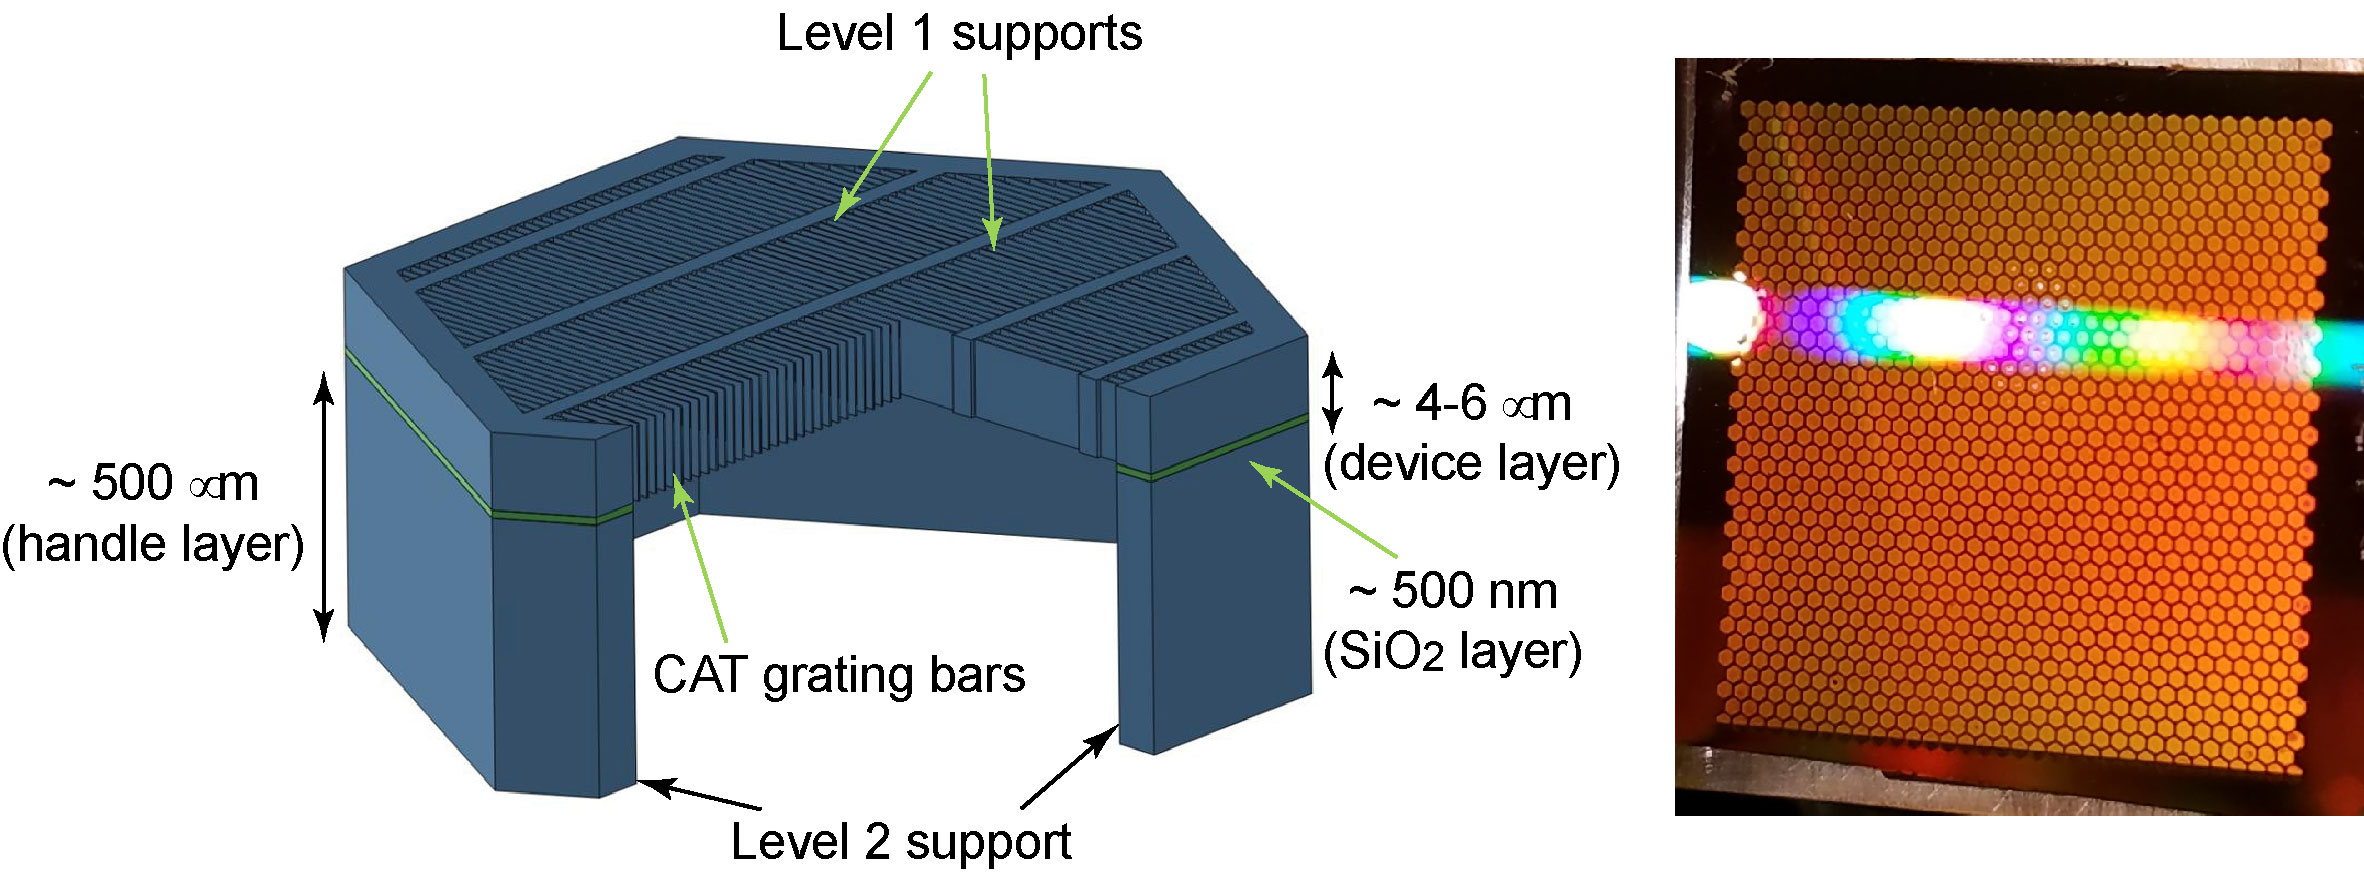
\includegraphics[height=5cm]{unitcell+pic.jpg}
\end{tabular}
\end{center}
\caption {\label{fig:cell}
Left: Schematic depiction of the structural hierarchy of the CAT grating membrane (see text). Right: Photograph of a back-illuminated $32\times32$ mm$^2$ prototype CAT grating membrane, showing the hexagonal L2 mesh and optical diffraction from the L1 mesh.
}
\end{figure}


The XGS is designed with a Rowland torus
geometry\cite{beuermann:78} where gratings are located on the
Rowland torus. The torus is tilted with respect to the optical axis\cite{doi:10.1117/12.856482,doi:10.1117/12.2273011}, see Figure~\ref{fig:sketch}. That way, gratings with the chosen blaze angle of 1.6~deg are still mostly tangential to the surface of the torus, minimizing the average distance between any point on the flat gratings and the surface of the torus. The torus dimensions are optimized to position the gratings close to the end of the mirror to increase the distance between the focal point and the dispersed signal, as this increases the spectral resolving power $R$.

\begin{figure} [ht]
\begin{center}
\begin{tabular}{c} %% tabular useful for creating an array of images
\includegraphics[width=\textwidth]{rowlandsketch.pdf}
\end{tabular}
\end{center}
\caption {\label{fig:sketch}
Layout of the AXIS/XGS. In both panels, the gray box on the left side indicates the mirror location; its focal point is at the intersection of the horizontal and vertical black lines. The drawing shows a cut through a plane, which contains the symmetry axis of the torus; two blue circles of radius $r$ show the intersection of this plane with the torus and blue dotted lines help to visualize the torus position. For the parameters chosen, the two circles overlap. $\alpha$ is chosen close to the blaze angle to make the blazed grating facets almost tangential to the Rowland Torus. Left: Conceptual sketch; right: to-scale.
}
\end{figure}

\subsection{Filters}

Since X-ray detectors are also sensitive to optical and UV light, we add an optical blocking filter of 30 nm Al topped with 10 nm of aluminum oxide, which may be directly deposited on the detectors. Above that, we simulate a 45~nm layer of Kapton mounted on a 95\% transmissivity metal mesh which acts as contamination filter to prevent contamination build-up on cold detector surfaces.


\subsection{Position of detector}
\label{sect:detpos}
\begin{figure} [ht]
\begin{center}
\includegraphics[height=6cm]{detectorplacement.pdf}
\end{center}
\caption {\label{fig:det}
Ray-trace of a continuum source through AXIS/XGS. CAT gratings disperse photons of different energy into different orders, such that most of them end up in a narrow range of angles. The photon distribution has a clear peak at twice the blaze angle, which we call the blaze peak. Detectors only need to cover this narrow region at 400-600~mm distance from the focal point of the mirror to catch the vast majority of photons.
}
\end{figure}
The geometry of CAT gratings favors diffraction orders that direct photons to a specific location (the ``blaze peak'') located 400-600~mm (Figure~\ref{fig:det}) from the focal point, where the detectors for the dispersed spectrum must be placed. The width of this peak depends on wavelength, the depth of the gratings, and the distribution of blaze angle (section~\ref{sect:blaze}) for each grating. To keep the cost and requirements on additional cooling, power, and data volume down, we simulate just 4 CCD-ID94 devices. Those CCDs are rectangular with 2048 times 1024 pixels of 24~$\mu$m size and together cover almost the entire blaze peak. In practice, one might want to use the same detector type that is also mounted in the imaging instrument in the focal plane to simplify integration and testing and later software development and calibration. Detector requirements for the dispersed signal are not very stringent: Since the signal is spread out, count rates are generally lower than in an imaging instrument, thus read-out can be slower and  24~$\mu$m pixels simulated here already oversample the line-spread function and there is no benefit of higher spatial resolution.

Detectors for the dispersed signal are mounted following the Rowland-torus geometry. The imaging detector at the focal point of AXIS, that is planned anyway, can provide information on the zero-order image position for wavelength calibration without placing any additional requirements on that detector.

\subsection{Ray-trace code}
\label{sect:raytrace}

We use the Python-based, open source, Monte-Carlo code MARXS for our ray-trace\cite{marxs1.1,2017AJ....154..243G}. The simulations for this work are run with a development version of MARXS to include AXIS-specific code; that version is publicly accessible in the MARXS repository with commit hash: 58b0d43f. Optical properties of materials such as diffraction or transmission probabilities are input from data tables and not calculated by MARXS itself.


\section{Results}
We study different configurations for AXIS and compare the effective area and resolving power. Some of the scenarios use gratings at a high TRL, very similar to what has been demonstrated for Arcus already, while others explore modifications that have not yet been demonstrated to the same level.

\begin{itemize}
  \item The baseline scenario studied here uses $30 * 60$ mm$^2$ flat gratings, where all gratings have exactly the same grating constant. They are arranged such that the short dimension is parallel to the dispersion direction and the long dimension to the cross-dispersion direction. About 1000 gratings are needed to cover the full aperture. In the following discussion and figures, simulations use this scenario unless otherwise noted.
  \item Using larger gratings means that fewer gratings are needed to cover the same geometric area which reduces cost and also losses due to geometric coverage by the grating support structure. A normal Si wafer can yield four $60 * 60$ mm$^2$ gratings, thus these can be manufactured at a similar cost as $30 * 60$ mm$^2$ gratings, but only half as many gratings have to be calibrated, mounted, and aligned.
  \item When gratings are flat, they deviate from the Rowland torus. This can be compensated by varying the grating period over the grating (``chirp''). Chirped gratings allow us to use very large gratings ($60 * 180$ mm$^2$) without loss of resolving power. Chirped gratings have not yet been demonstrated. In principle, the chirp needed is different for every grating, but in practice, just two or three types of gratings will suffice\cite{10.1117/12.2562878}, keeping complexity and cost down and the total number of gratings is only about 150 to cover the entire aperture.
  \item Alternatively, the gratings can be bent in at least one dimension to follow the Rowland-torus more closely. Laboratory tests of (smaller) bent gratings indicate that the bending does not impact their throughput\cite{10.1117/12.2274205}. Bending is only worth the effort is large gratings are used, here $60 * 60$ mm$^2$.
  \item Finally, we present simulations where the PSF is dominated by alignment error (the ``round PSF'' scenario described in Sect.~\ref{sect:PSF}). A round PSF is the worst-case for a grating spectrometer, because there is no benefit of subaperturing (using only a fraction of mirror aperture, chosen such that the resulting PSF is asymmetric and the dispersion direction is selected to make the spectral features narrow in dispersion direction), but we adjust the in-plane and out-of-plane scatter to keep the total mirror PSF at 1 arcsec HPD. Gratings are arranged as in the baseline scenario.
\end{itemize}


\subsection{A detailed look at the diffraction of 0.6 keV photons}
First, we simulated events at one specific energy close to the crucial O~{\sc vii} triplet at 2.1~nm and see how the diffracted orders look on the detector and what we can learn from subaperturing.

Figure~\ref{fig:blaze} shows the distribution of blaze angles for the different scenarios. The position of the detectors is optimized for a specific blaze angle. For flat gratings of finite size, the blaze angle is set for the central ray. That means that photons of a converging beam that pass the grating in a different location will have a different value for the blaze angle. The larger the grating, the larger the range of blaze angles. This leads to broader blaze peak (Fig.~\ref{fig:det}) and photons will be lost unless the read-out detector is expanded. Bending the gratings with a radius of 8.5~m (the average distance of a grating from the focal point) reduces the spread of blaze angles to ensure that all photons intersect the grating at the blaze angle that gives the best diffraction efficiency.
\label{sect:blaze}

\begin{figure} [ht]
  \begin{center}
  %\begin{tabular}{c} %% tabular useful for creating an array of images
  \includegraphics[width=0.8\textwidth]{blaze}
  %\end{tabular}
  \end{center}
  \caption {\label{fig:blaze}
    Distribution of blaze angles over all gratings for different grating sizes. For the bent gratings, all photons fall into the same bin, which is cut-off in the figure for display purposes.
  }
\end{figure}

\subsection{Line spread function and subaperturing}
\label{sect:LSF}
We define the resolving power as: $R = \frac{\lambda}{\Delta \lambda} =
\frac{d_x}{FWMH}$ where $\lambda$ is the wavelength of a spectral line with negligible intrinsic width, and $\Delta \lambda$ is the observed width (the ``Line spread function (LSF)'') of this feature. The $FWMH$ is the full width at half maximum of the event distribution, measured in the dispersion direction, and $d_x$ is the distance between the center of a diffracted order and the center of the zeroth order.

\begin{figure} [ht]
\begin{center}
%\begin{tabular}{c} %% tabular useful for creating an array of images
\includegraphics[width=0.8\textwidth]{orders.pdf}
%\end{tabular}
\end{center}
\caption {\label{fig:orders}
  \emph{Left:} Position of gratings in the aperture plane. The gratings are color coded by angle relative to the dispersion direction (black arrow).
  \emph{Other panels:} Distribution of photons with exactly 0.6~keV in the sixth order for different CAT grating sizes and mirror scattering properties. Each dot represents a single detected photon, color coded by the grating it passed. Note that the x and y axes are on different scales.
}
\end{figure}

Figure~\ref{fig:orders} shows the distribution of 0.6~keV photons diffracted
into the $6^{\rm th}$ order on the detector for our scenarios.
The left plot in the figure shows the position
of the gratings in the mirror aperture plane. Gratings are colored according to the
\textbf{azimuthal} angle from the dispersion direction. The Rowland torus is symmetric to reflection on the dispersion axis ($y=0$ line in the figure) and this is represented in the color of the gratings in the panel.
In the other panels, photons are colored according to the grating they passed through. Photons going through gratings with different azimuthal angles have different spatial distributions on the detector.
Photons that went through the gratings displayed in purple are distributed narrower than the red points; using only the former photons will deliver a lower $FWHM$ and thus higher $R$.

When the spectrum is extracted for analysis, the distribution in cross-dispersion direction ($y$-axis in figure~\ref{fig:orders}) does not matter for the width of the spectral feature. Figure~\ref{fig:howtosubaperture} shows the photon distributions in figure~\ref{fig:orders} collapsed on the dispersion axis. To understand how subaperturing (filling only part of the aperture with gratings) can influence $R$, the figure displays the photon distribution resulting from gratings in narrow sectors, e.g. a pie-shaped sector containing just photons that pass through gratings with an absolute azimuthal angle of 30-60~degrees (light blue line in Figure~\ref{fig:howtosubaperture}, corresponding to the light blue gratings in figure~\ref{fig:orders}, left).

\begin{figure} [ht]
  \begin{center}
  %\begin{tabular}{c} %% tabular useful for creating an array of images
  \includegraphics[width=0.4\textwidth]{howtosuabperture.pdf}
  %\end{tabular}
  \end{center}
  \caption {\label{fig:howtosubaperture}
    Distribution of detected photons in the dispersion direction for different subaperture angles. The flux is shown with a different, arbitrary normalization for each panel. The zero point of the $x$-axis is set to be the center of the simulated distribution. This is the same data as in Figure~\ref{fig:orders}, but displayed as a histogram along the cross-dispersion direction; the colors of the lines in this figure match the colors of the gratings in the left panel of Figure~\ref{fig:orders}.
  }
\end{figure}

For all the scenarios, the photons passing through gratings located close to perpendicular to the dispersion direction (light green line) have the sharpest peaks. The other lines differ from the green line in two ways: They are often wider and in some cases their peaks are shifted. The width of the distribution is due to the intrinsic mirror PSF and the fact that the gratings deviate from the Rowland torus. In our simulations, the gratings are placed such that the center of each grating matches the Rowland torus. Because of the tilt of the torus, gratings located in the range $60-90^\circ$ are almost tangential to the torus surface and have the smallest average deviation and thus the sharpest LSF. Larger gratings have larger average deviations than smaller gratings and thus the green LSF in the $60\;\mathrm{mm}\times 30\;\mathrm{mm}$ scenarios is narrower than in the $60\;\mathrm{mm}\times 60\;\mathrm{mm}$ scenario. Gratings located at larger or smaller angles cannot be tangential because they have to be rotated to match the blaze angle specification and deviate more from the surface of the torus, leading to wider LSFs (lower $R$). Thus, these simulations show that a higher $R$ can be achieved if only certain parts of the aperture are filled with gratings. As the size of the grating increases, the spots get wider and $R$ is reduced, unless gratings are chirped or bent.

A second effect is the shift in the peak of the LSF between the green line and the other angles' ranges; this is due to the fact that for gratings tangential to the Rowland torus, the average distance of the grating to the detector is larger than for gratings that intersect the Rowland torus. The latter is required in some locations to keep the blaze angle in the specified range.


The two scenarios $60\;\mathrm{mm}\times 30\;\mathrm{mm}$ and $60\;\mathrm{mm}\times 30\;\mathrm{mm}$ (scatter) use the same gratings, but differ in the scatter properties of the mirror. If the mirror PSF is dominated by figure errors and scattering, then subaperturing will increase $R$ a lot more than in the scenario where the PSF is dominated by off-center errors (``PSF round'').

\begin{figure} [ht]
  \begin{center}
  \begin{tabular}{c} %% tabular useful for creating an array of images
  \includegraphics[height=6cm]{traderaeff.pdf}
  \end{tabular}
  \end{center}
  \caption {\label{fig:trade}
  Each colored line in this plot is one scenario (grating size, chirp yes/no etc.). The line connects simulations with different subaperturing angle and specific angles are marked with dots (top to bottom filling 100, 83, 67, 50, 33, and 17 \% of the total space with gratings). This figure corresponds to an energy of 0.6~keV.
  }
\end{figure}

Figure~\ref{fig:trade} shows the trade-off between effective area and $R$ for different fractions of the aperture filled with gratings and different scenarios. Of the five scenarios studied, large, chirped gratings provide the best performance, but also require the most development in grating manufacturing. Without chirping, smaller gratings provide better $R$, but a lower effective area than larger gratings.  Comparing the two scenarios $60\;\mathrm{mm}\times 60\;\mathrm{mm}$  (orange) and $60\;\mathrm{mm}\times 60\;\mathrm{mm}$ (bent - purple), we can see that the bent gratings achieve a better effective area for a given filling factor, because all photons interact with the grating at the same blaze angle, but $R$ suffers because the bent gratings deviate more from the Rowland torus then flat gratings.
For all scenarios, we can choose to populate only part of the aperture with gratings, reducing the effective area and increasing $R$. That choice has to be made based on the science requirements for high-resolution grating spectroscopy.

\subsection{Resolving power and effective area}
To evaluate the resolving power and effective area for a range of photon energies we run ray-traces for the canonical case of $30 * 60$~mm gratings with no bending or chirping. In this early phase of the design, we limit ourselves to a coarse wavelength grid and thus to not resolve all details like chip gaps.

\begin{figure} [ht]
  \begin{center}
  %\begin{tabular}{c} %% tabular useful for creating an array of images
  \includegraphics[width=0.8\textwidth]{RAeff}
  %\end{tabular}
  \end{center}
  \caption {\label{fig:RAeff}
    Effective area (\emph{left}) and resolving power (\emph{right}) for different subaperturing angles in the baseline scenario.
  }
\end{figure}

Figure~\ref{fig:RAeff} shows the effective area and resolving power $R$. The latter is essentially constant with wavelength, because photons are all diffracted into the blaze peak and for a given spectrograph and mirror, $R$ just depends on the distance between the focal point and the diffracted order.
The effective area of the diffracted signal increases above about 1.2~nm where the Si grating bar side walls reflect the photons efficiently. The deep dip around 2~nm is due to one of the two or three relevant orders hitting a chip gap. However, since we see more than one diffraction order for most wavelengths, some signal is still available. Chip gaps can further be mitigated through dithering or placing the source in a specific location to avoid spectral regions of interest to fall on chip gaps. There should be more chip gaps, but the wavelength resolution of the simulations here is so low that most of them are just stepped over.


\section{Cost and technical readiness level}
The XGS requires two new systems to be added to AXIS: Gratings and detectors. The requirements on the detectors are relatively simple and detectors can be chosen from a variety of CCDs with high flight heritage or could be chosen to match the detectors used for direct imaging. In that way, there is additional cost to procure the detectors, but no impact on the technology maturation plan for AXIS, only minimal software development for grating data reduction, and no added technical risk.

CAT gratings have been matured for the Lynx and Arcus/MIDEX mission concepts and have been tested in a flight-like configuration including alignment of several grating elements in a grating holder\cite{2022ApJ...934..171H}. As such, we assess the technology at TRL 6 for small flat gratings; minor development is needed to reach TRL 6 if other grating parameters are chosen (size, depth, width of the grating bars, bending, chirping).

Both the Arcus and the Lynx mission efforts developed detailed production plans, schedules, and cost estimates for CAT gratings. Based on those detailed numbers, we can make a rough estimate for the total cost of AXIS with the XGS configuration presented in this work (including gratings, holders, insertion mechanism, detectors, calibration, software development) to be just a few percent the total cost of the AXIS mission.
Since the marginal cost of manufacturing additional gratings is small and the same number of detectors will be needed in any case, the cost does not change much if only part of the aperture is covered with gratings.

\section{Discussion}
We have shown through ray-tracing that AXIS/XGS can reach $R>6000$ with an effective area around 500~cm$^2$ in the conservative case of covering just 33\% of the aperture with CAT gratings in the baseline scenario. AXIS can reach an effective area around 1500~cm$^2$ at $R=4000$, if the entire aperture is covered. With this design, AXIS/XGS will outperform all existing or accepted future X-ray missions by a wide margin. The CAT gratings simulated here are straightforward modifications of gratings that have already been manufactured and been aligned and tested in an X-ray beamline\cite{2022arXiv220609013H}; the total efficiency of the gratings simulated here, is about a factor of two better than the gratings that were planned for the Arcus MIDEX mission. The improvement is a sum of several small steps (larger grating facets to reduces dead area from mounting structures, deeper gratings, wider distances between support structures, thinner gratings bars and support structures), some of which are well underway now, e.g.\ deeper gratings have already been tested in an X-ray beamline and been shown to reach the $R$ values required\cite{2022arXiv220609013H}. Still, in the unlikely case that none of the improvements succeed, the predicted effective area could be up to a factor two lower than the numbers given above.

Considering energies of 0.5~keV as an example, the AXIS/XGS with 33\% coverage of the aperture will have about 40 times the effective area and at least 10 times the resolving power of Chandra/LEGTS; it will have two orders or magnitude more effective area than Chandra/HETGS at launch and almost four orders of magnitude more than Chandra/HETGS has today and a factor of 5 better resolving power\cite{2005PASP..117.1144C}; and compared to XMM/RGS our ray-traces show more than one order of magnitude increase in $R$ and about one order of magnitude in effective area.
%The proposed Arcus mission plans for $R$ and effective area 2-3 times lower than what AXIS/XGS can deliver\cite{doi:10.1117/12.2273011}.
Microcalorimaters such as those on XRISM\cite{10.1117/12.2565812} and Athena X-IFU do not reach above $R=200$ at low energies, a critical bandpass for diagnosing plasma temperature and density for 'soft' X-ray sources such as young pre-main sequence stars. Such a dramatic jump in capability will lead to significant new discoveries in many areas in astrophysics.

Further refinements of the design shown here can be made, but the most important input is to set the science requirements on $R$ and effective area to decide on the subaperturing angle. Options for the CAT gratings with lower TRL include a coating with a metal like Pt which will increase the reflectivity at higher energies and increase the energy range where $R=5000$ is possible to 2~keV, and bending and chirping as simulated above. For the design of the spectrograph, we can optimize the tilt of the Rowland torus or split gratings such that dispersed gratings fall on different channels like the HEG and MEG in Chandra/HETG\cite{2005PASP..117.1144C}: A third of the aperture could be covered with gratings to reach $R>6000$ with an effective area around 500~cm$^2$, while the remaining area could be covered with gratings that diffract in slightly different direction, so that another 1000~cm$^2$ effective area are simultaneously available at a $R>3000$ - still a factor of a few more than any existing instrument.

While not simulated in this work, CAT gratings allow relatively easy alignment tolerances which can be met by machining alone in many degrees of freedom. Ref~\citenum{10.1117/1.JATIS.5.2.021003} found that $1\sigma$ tolerances are typically several mm for translations and arcminutes or even degrees for rotations. AXIS/XGS has a larger mirror PSF than used in that study, so $R$ will be lower than it would have been for Lynx/XGS\cite{10.1117/1.JATIS.5.2.021003} anyway, and thus alignment requirements for AXIS/XGS would be even looser.




% Note add recent SPIE citations for chirp etc.



\section{Summary}
In this article, we present a concept for an X-ray grating spectrometer (XGS) for the AXIS probe. Based on CAT grating technology that has been developed and matured over the last decade or so, the spectrometer can deliver a resolving power $R=5000-7000$ and an effective area up to 2000~cm$^2$ in the soft X-ray band (1.5-3.5~nm) for potentially several dozen sources in the field of view depending on their location in the sky and roll angle of the telescope. It is important to note that CAT grating based spectrometers have fairly loose alignment requirements that can be met by machining alone in many degrees of freedom\cite{10.1117/1.JATIS.5.2.021003}, reducing time-consuming and costly alignment steps. Effective area and $R$ for the AXIS/XGS are orders of magnitude better than existing instruments and will open entirely new science areas such as the detection of weak absorption lines in the warm-hot intergalactic medium, determining elemental abundances in proto-planetary disks through absorption edges, and kinematically resolving emission lines from accretion and winds in stars.

The XGS requires two new elements to be introduced to the AXIS design: CAT gratings just behind the mirror, and detectors for the dispersed light in the focal plane. The TRL for both components is high and the total cost of the XGS would be just a few percent of the total budget. The gratings are mostly transparent at higher energies, but could also be moved into and out of the beam as in the highly successful Chandra gratings, so there would be no impact at all on observations that do not specifically request dispersed spectra. Moreover, observations with the gratings inserted will simultaneously provide undispersed (0th order) images with the standard imaging detectors on AXIS. We present different design options based on different grating sizes and there is a trade-off where more development of larger bend or chirped gratings can improve performance and reduce cost, but we show that all designs studied provide unmatched scientific opportunities in the soft X-ray band.




\acknowledgments
Support for this work was provided in part through NASA grant NNX17AG43G and Smithsonian Astrophysical Observatory (SAO)
contract SV3-73016 to MIT for support of the {\em Chandra} X-Ray Center (CXC),
which is operated by SAO for and on behalf of NASA under contract NAS8-03060.
The simulations make use of Astropy, a community-developed core Python package
for Astronomy\cite{2013A&A...558A..33A,astropy}, numpy\cite{numpy}, and
IPython\cite{ipython}. Displays are done with matplotlib\cite{matplotlib}.


\subsection*{Biographies}
\vspace{2ex}\noindent\textbf{Hans Moritz G\"unther} is a research scientist at MIT. He received his undergraduate degree (in 2005) and his PhD (in 2009) in physics from the University of Hamburg, Germany. After that, he worked at the Harvard-Smithsonian Center for Astrophysics and came to MIT in 2015. He is currently the lead developer of MARX, the ray-tracing software used for the Chandra X-ray observatory. His science interests are in star formation using data from the radio to X-rays.


\vspace{2ex}\noindent\textbf{David Principe} is a research scientist at MIT. He earned his Bachelor's of Science degree in astrophysics (2009) from Ohio University and his Ph.D. (2014) from the Rochester Institute of Technology. After a two-year postdoctoral research fellowship at the Universidad Diego Portales in Santiago, Chile, he became a post doctoral research associate at MIT. His current work as a research scientist involves supporting the Chandra X-ray Observatory and studying young stellar evolution.


\vspace{1ex}
\vspace{2ex}\noindent\textbf{Ralf K.~Heilmann} is a principal research scientist at the MIT Kavli Institute for Astrophysics and Space Research, and the associate director of the Space Nanotechnology Laboratory (SNL).  He received his Diplom in physics from the FAU Erlangen/N\"urnberg (1991), and his MS (1993) and PhD (1996) in physics from Carnegie Mellon University.  After a postdoc at Harvard he joined the SNL and has since focused on advanced lithography and the development of x-ray optics for astronomy.


\vspace{1ex}
\vspace{2ex}\noindent\textbf{Peter Cheimets}: Business development lead and head of SAO's SmallSat program: He received his BS in mechanical engineering in 1974 from MIT, MS in dynamics and controls in 1981 from Stanford, and a Masters of Science in engineering management in 2007 from Tuft University. He has developed EUV and X-ray missions for the Smithsonian Astrophysical Observatory for 25 years.

\vspace{1ex}
\vspace{2ex}\noindent\textbf{Edward Hertz} is a Project/Mechanical Engineer at SAO with over 30 years of experience in the design and development of complex instruments used for astronomical and astrophysical data collection.  He has directed the efforts of multi-disciplined engineering and technical teams from project conception through optical alignment and subassembly integration.  He received his BS in mechanical engineering with a minor in engineering management from Tufts University in 1983.


\vspace{1ex}
\vspace{2ex}\noindent\textbf{Randall Smith} is the Associate Director - Science at the Center for Astrophysics $|$ Harvard \& Smithsonian, and leader of a number of X-ray grating mission proposals. His science interests include understanding the formation and evolution of galaxies as well as the interstellar medium and the physics of hot plasma emission.


%%%%% References %%%%%

\bibliographystyle{spiejour}   % makes bibtex use spiejour.bst
\bibliography{refs2}   % bibliography data in report.bib


%%%%% Biographies of authors %%%%%


\listoffigures
\listoftables

\end{spacing}
\end{document}